\section{Advent of Flutter}
Google introduced Flutter for native app development. Built using Dart,C, C++ and Skia, Flutter is an open-source, multi-platform app UI framework. Prior to Flutter 2.0, developers could only target Android, iOS and the web. Flutter 2.0 released support for macOS, Linux, and Windows as a beta feature. Flutter 2.10 released with production support for Windows and Flutter 3 released production support for all desktop platforms. It provides a framework, widgets, and tools. This framework gives developers a way to build and deploy mobile, desktop, and web apps. Flutter works with Firebase and supports extending the framework through add-ons called packages. These can be found on their package repository, pub.dev. JetBrains also supports a Flutter plugin\cite{enwiki:1155641282}.

\begin{figure}[H]
    \centering
    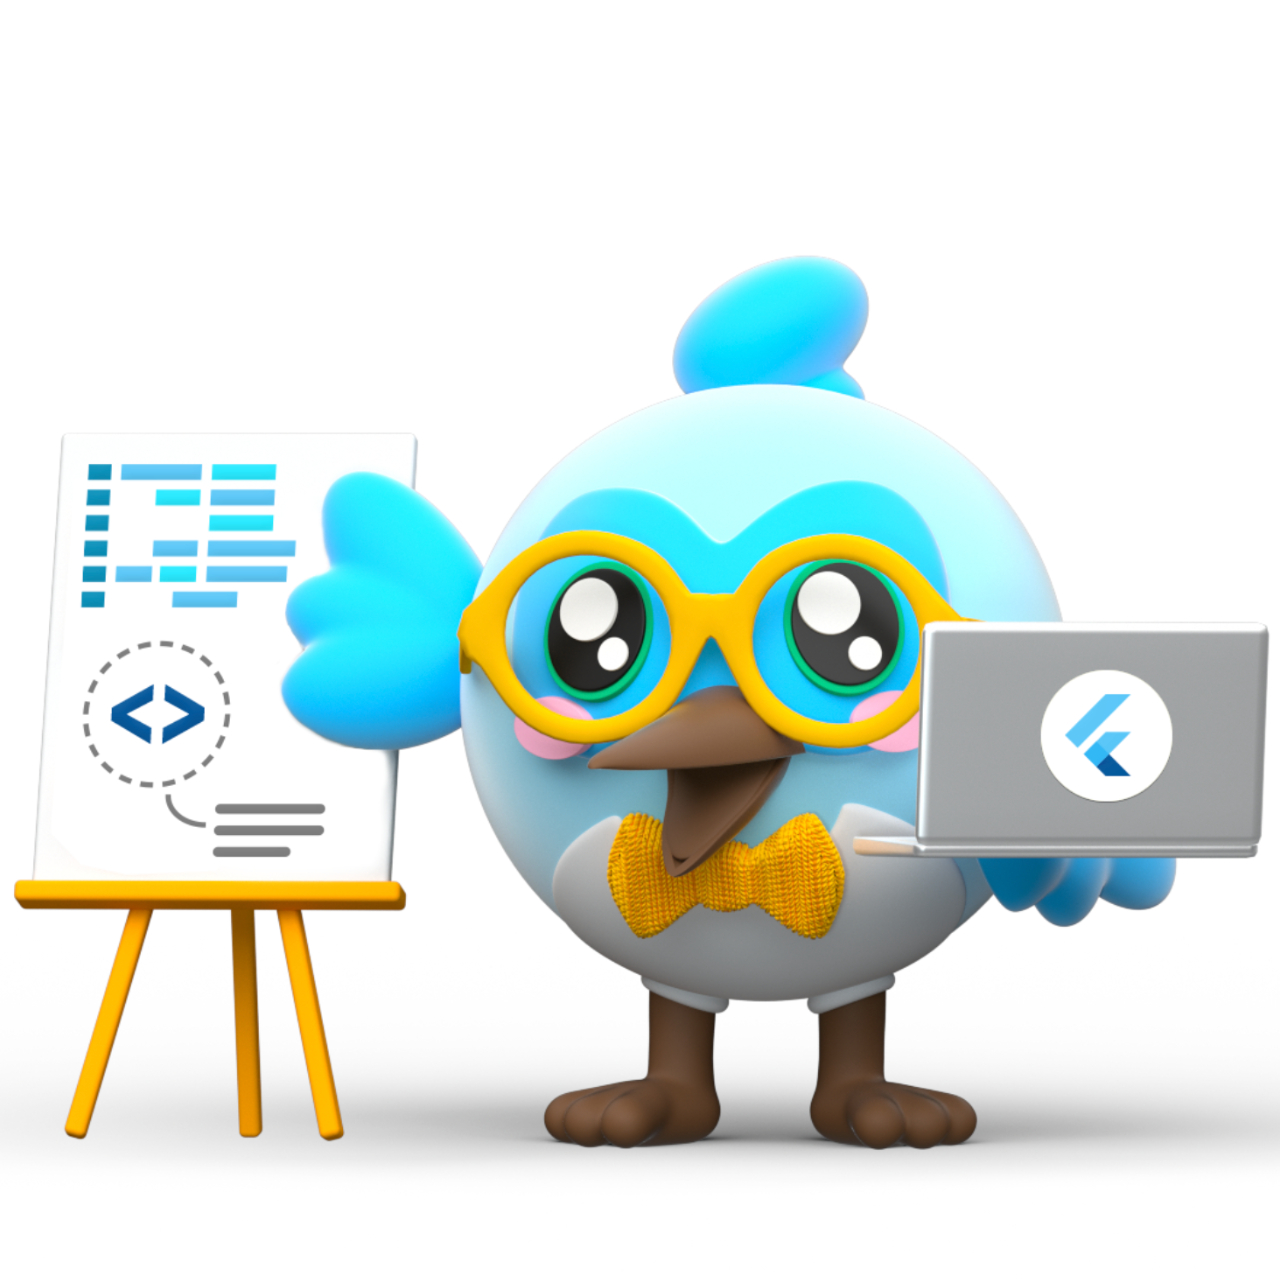
\includegraphics[scale=0.25]{media/dash.jpg}
    \caption{Flutter Mascot (Dash)}
    \label{fig:dash}
\end{figure}
